%!TEX root = ../stoeter_sourcecount.tex
% chktex-file 46
% chktex-file 45

\section{Problem Formulation}%
\label{sec:problem_formulation}
% introduce the section
We consider the task of estimating the maximum number of concurrent speakers \( \cardinality \in \mathbb{Z}^{+}_{0} \) in a single-channel audio mixture \(\mathbf{x}\).
This is achieved by applying a mapping from \(\mathbf{x}\) to \(\cardinality \).
We now provide details on the notations, the general structure of the method, and various ways to exploit the deep learning framework to estimate \(\cardinality \).

\subsection{Signal Model}%
\label{ssec:signal_model}
Let \(\mathbf{x}\) be a vector with \(N\) discrete time samples, representing a linear mixture of \(L\) single speaker speech signal vectors \(\mathbf{s}_l\).
The value observed at sample~\(n\) for the mixture is given by~$x_n$ and for the individual speech segments by~$s_{nl}$.
The mixture then results in
%
\begin{equation}
  x_n = \sum_{l=1}^{L}{s_{nl}} \; \forall n \in \mathbb{Z}^N.
  \label{eq:mixing_model}
\end{equation}
%
Naturally, each speaker~$l=1,\dots,L$ is not active at every time instant.
On the contrary, we assume there is a latent binary \textit{speech activity} variable~$v_{nl}\in \left\{ 0,1 \right\}$ that is defined as:
\begin{equation}
v_{nl}=\begin{cases}
1 & \text{if }\left|s_{nl}\right|>0\\
0 & \text{otherwise}.
\end{cases}\label{eq:definition_speech_activity}
\end{equation}

Our objective of estimating the maximum number of concurrent speakers can now be formulated as
%
\begin{equation}
k=\underset{n}{\max}\left(\sum_{l = 1}^{L} v_{nl}\right) \; n \in \{ 1,\ldots, N \}
\label{eq:definition_k}.
\end{equation}
%
As can be seen, our proposed task of estimating $k\leq L$, is more closely related to source separation whereas the estimation of \(L\) is more useful for tasks where speakers do not overlap.
For instance, three non-overlapping speakers would result in \(L = 3\) and \(\cardinality = 1\).
In the rest of this work, we assume that no additional prior information about the speakers is given to the system except possibly the maximum number of concurrent speakers~$k_{\max}$, that is application-dependent and represents an upper bound for the estimation.

While speaker diarization would mean estimating the whole speech activity matrix~$v_{nl}$ in~(\ref{eq:definition_speech_activity}), our problem of estimating only~$k$ in~(\ref{eq:definition_k}) is more abstract as it requires a direct estimation of the count as advocated in Section~\ref{sec:introduction}.
\begin{figure}[t]
  \centering
  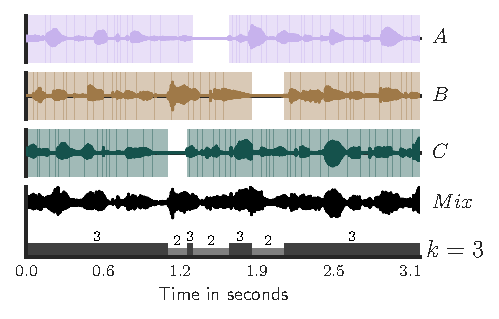
\includegraphics[width=0.8\columnwidth]{Chapters/dsc/figures/teaser.pdf}
  \caption{Illustration of our application scenario of three concurrent speakers (A, B, C) and their respective speech activity. Bottom plot shows the mixture (input), the number of concurrently active speakers and its maximum \(k\) which is our targeted output.}%
  \label{fig:teaser}%
\end{figure}
In Figure~\ref{fig:teaser}, we illustrate our setup in a ``cocktail-party'' scenario featuring~$L=3$ unique speakers.
At any given time, we see that at most~$k=L=3$ speakers are active at the same time and~$k=2$ could be the outcome if a smaller excerpt would be evaluated.

Now, the system we propose is actually not inputting the signal vector $\mathbf{x}$, but rather a Time-Frequency (TF) representation as the absolute value of the Short-Term Fourier Transform of~$\mathbf{x}$ that is denoted by $\mathbf{X}$.
In the following, $\mathbf{X}$ is the non-negative input for the system.

\subsection{Probabilistic formulation}%
\label{ssec:model}
In a supervised scenario, let~$ \left\{\mathbf{X}_t,k_t\right\}_t$ be all of our learning examples, where~$t \in{1,\dots,T}$ denotes the $t$-th training item from the training database.
For the purpose of learning a mapping between~$\mathbf{X}$ and~$k$, we adopt a probabilistic viewpoint and introduce a flexible generative model that explains how a particular source count~$k$ corresponds to some given input ~$\mathbf{X}$.

First, we consider that all training samples~$\left\{\mathbf{X}_t,k_t\right\}_t$ are independent.
For each sample, we consider that~$k_t$ is drawn from a probability distribution of a known parametric family, parameterized by some latent and unobserved parameters~$\mathbf{y}_t$
\begin{equation}
\mathbb{P}\left(k_{t}\mid\mathbf{X}_{t}\right)=\mathcal{L}\left(k_{t}\mid \mathbf{y}_{t}\right),
\end{equation}

% @soumitro
% \begin{equation}
% k_{t} \sim \mathcal{P}(k_{t} | \mathbf{y}_{t})
% \end{equation}

the distribution~$\mathcal{L}\left(\cdot\mid \mathbf{y}_{t}\right)$ is called the \textit{output distribution} in the following.
We further assume that there is some deterministic mapping between~$\mathbf{X}_t$ and~$\mathbf{y}_t$, embodied as
\begin{equation}
\mathbf{y}_{t}=f_{\mathbf{\theta}}\left(\mathbf{X}_{t}\right),
\end{equation}
where $\mathbf{\theta}$ are the parameters for this deterministic mapping, that is independent of~$t$. This results in an output distribution given by
\begin{equation}
\mathbb{P}\left(k_{t}\mid\mathbf{X}_{t}\right)=\mathcal{L}\left(k_{t}\mid f_{\mathbf{\theta}}\left(\mathbf{X}_{t}\right)\right).\label{eq:output_distribution}
\end{equation}
Assume for the rest of this section that these parameters~$\mathbf{\theta}$ are known.
Given a previously unseen input~$\mathbf{X}$, expression~(\ref{eq:output_distribution}) means we can compute the distribution of the source count~$k$.
% The advantage of that probabilistic formulation is to introduce some flexibility instead of enforcing a more classical deterministic mapping such as~$k_{t}=f_{\mathbf{\theta}}\left(\mathbf{X}_{t}\right)$.

The objective of our counting system is to produce a point estimate~$\hat{k}$ rather than a whole output distribution~$\mathbb{P}\left(k\mid\mathbf{X}\right)$.
A first option is to pick as an estimate the most likely outcome for the output distribution, thus resorting to Maximum A Posteriori (MAP) estimation:
\begin{equation}
\hat{k}=\underset{k}{\text{argmax}}\ \mathcal{L}\left(k\mid f_{\mathbf{\theta}}\left(\mathbf{X}\right)\right).
\end{equation}

However, MAP is not the only option and a broad range of point estimation techniques may be obtained when resorting to decision theory~\cite{berger1985}.
We may for example also choose~$\hat{k}$ as the value that minimizes the marginal average cost of choosing an estimate $\hat{k}$ instead of the true value $k$, when $k$ is distributed with respect to the output distribution
\begin{equation}
\hat{k}=\underset{u}{\text{argmin}}\intop_{k}d\left(k,u\right)\mathcal{L}\left(k\mid f_{\mathbf{\theta}}\left(\boldsymbol{X}\right)\right) \mathrm{d} k,\label{eq:estimate_hatk}
\end{equation}
where $d\left(k,u\right)$ is the cost of picking $u$ as an estimate when the true value is~$k$.
It may be any function that seems appropriate, not restricted to the subject of differentiability.
% For instance, when we take~$d\left(k,u\right)=\left|k-u\right|^{2}$, we obtain the Minimum Mean Squared Error (MMSE) estimate.
However, we retain the more general formulation~(\ref{eq:estimate_hatk}) because other choices will sometimes prove more effective, as we show later.
For notational convenience, we write~(\ref{eq:estimate_hatk}) as
\begin{equation}
\hat{k}=q\left(f_{\mathbf{\theta}}\left(\boldsymbol{X}\right)\right),
\end{equation}
and $q\left(\cdot\right)$ is called the~\textit{decision function}.
Using this strategy, we have everything to produce a single source count estimate~$\hat{k}$ from input features~$\mathbf{X}$, provided the parametric family~$\mathcal{L}$ and the mapping $f_{\mathbf{\theta}}$ as well as its parameters $\mathbf{\theta}$ are known.

In this study, we choose a deep neural network for the mapping $f_{\mathbf{\theta}}$, whose weights~$\mathbf{\theta}$ are trained in a supervised manner.
Once a particular network architecture has been chosen, learning its parameters is achieved through classical stochastic gradient descent.
If we assume that the particular family~$\mathcal{L}$ of output distributions has been chosen, it appears natural to learn the parameters~$\mathbf{\theta}$ that maximize the likelihood of the learning data.
More specifically, the total cost to be minimized becomes
\begin{equation}
C=\sum_{t=1}^{T}-\log\mathcal{L}\left(k_{t}\mid f_{\theta}\left(\boldsymbol{X}_{t}\right)\right).\label{eq:total_cost}
\end{equation}
The derivative of this cost (\ref{eq:total_cost}) with respect to the parameters can be used to learn the network parameters.
\par
Three different choices for the family of output distributions (classification, Gaussian regression and Poisson regression) as well as the corresponding decision functions~$q\left(\cdot\right)$ were investigated and discussed in~\cite{stoeter17}, and the reader is referred to it for further details.


% \subsubsection{Classification}
%
% In a classification setting, the output distribution is directly taken as \textit{discrete}, discarding any meaning concerning the ordering of the different possible values.
% In other words, \(\cardinality \) may only take a finite set of values, whose actual labelling is not assumed to bear any particular information.
% In that case, the output distribution~$\mathcal{L}\left(k\mid f_\mathbf{\theta}\left(\mathbf{X}\right)\right)$ is taken as multinomial with~$L+1$ (when we assume that \(k\) can be 0) classes.
% Given some particular input~$\mathbf{X}$, the network generates the posterior output probability for each of those \((L + 1)\) classes, and a MAP decision function may for instance be chosen that simply picks the most likely class:
%
% \begin{equation}
% \hat{k}=q\left(f_{\mathbf{\theta}}\left(\mathbf{X}\right)\right)=\arg\max\mathcal{L}(k\mid f_{\mathbf{\theta}}\left(\mathbf{X}\right)).
% \end{equation}
%
% Notwithstanding its conceptual simplicity, classification has two drawbacks.
% First, the intuitive ranking between different estimates is lost: e.g. \(p(\cardinality = 6) \) may not depend on \(p(\cardinality = 5) \).
% Second, the largest possible count $L$ is given \textit{a priori}.
% Despite these limitations, classification based approaches have successfully been applied in deep neural networks for counting objects~\cite{segui15, zhang2015salient, khan16} in images.
%
% \subsubsection{Gaussian Regression}
% Compared to classification, where the ordering of $k\in\mathbb{N}$ is not at all taken into account, adopting a strategy where~$k$ derives from an output distribution defined on the real line seems like a desirable setup.
% However, this strategy comes with the additional difficulty of handling the fact that~$k$ is integer.
% To circumvent it, we take $k$ as the rounding of a latent variable $f_{\mathbf{\theta}}\left(\mathbf{X}\right)\in\mathbb{R}$, and exploit the fact that rounding may be efficiently modelled as introducing white additive Gaussian noise, so that we may write:
% \begin{equation}
% k\sim\mathcal{N}\left(f_{\mathbf{\mathbf{\theta}}}\left(\mathbf{X}\right),\Delta\right),\label{eq:AWGN_model}
% \end{equation}
% where $\mathcal{N}$ is the Gaussian scalar distribution and $\Delta$ is the rounding noise variance, that is independent of any model parameters but only depends on the fact that $k$ is the integer closest to $f_{\mathbf{\mathbf{\theta}}}\left(\mathbf{X}\right)$.
%
% As can be seen, the output distribution in that setting becomes the Gaussian and the associated cost function is the classical squared error.
% During inference and given the output~$f_{\mathbf{\mathbf{\theta}}}\left(\mathbf{X}\right)$ of the network, the best discrete value that is consistent with the model is simply the rounding operator $\left[\cdot\right]$:
%
% \begin{equation}
% \hat{k}=\left[f_{\mathbf{\mathbf{\theta}}}\left(\mathbf{X}\right)\right].
% \end{equation}
%
% Gaussian regression has achieved state-of-the-art counting performance in computer vision using deep learning frameworks~\cite{zhang15, arteta16, marsden16, boominathan16}.
%
% \subsubsection{Discrete Poisson modelling}
% When it comes to modelling count data, it is often shown effective to adopt the Poisson distribution.
% First, this strategy retains the advantage of the classification approach to directly pick a probabilistic model over the actual discrete observations, avoiding the somewhat artificial trick of introducing a latent variable that would be rounded to yield the observation.
% Second, that model retains the algebraic structure of $k\in\mathbb{N}$ and thus avoids the inconvenient of the classification approach to completely drop dependencies between classes.
%
% Due to these advantages, the Poisson distribution already enjoyed some use in studies devising deep architectures for counting systems~\cite{Rezatofigh16}.
% In~\cite{fallah09, chan09, Rezatofigh16} it is for instance shown that the number of objects in images can be well modelled by the Poisson distribution. Inspired by these previous work, we also consider the Poisson output distribution:
% \begin{equation}
% \mathbb{P}\left(k\mid f_{\mathbf{\theta}}\left(\mathbf{X}\right)\right)=\mathcal{P}\left(k\mid f_{\mathbf{\mathbf{\theta}}}\left(\mathbf{X}\right)\right),
% \end{equation}
% where $\mathcal{P}\left(\cdot\mid\lambda\right)$ denotes the Poisson distribution with scale parameter~$\lambda$.
%
% In that setup, the cost function at learning time is the Poisson negative log-likelihood and the deep architecture at test time provides the predicted scale parameter $f_{\mathbf{\mathbf{\theta}}}\left(\mathbf{X}\right)\in\mathbb{R}_+$, which summarizes the whole output distribution.
%
% As a decision function~$q$ in that setting, we considered several alternatives. A first option is to again resort to MAP estimation and pick the mode $\left[f_{\mathbf{\mathbf{\theta}}}\left(\mathbf{X}\right)\right]$ of that distribution as a point estimate. However, experience showed that this is not the best choice. After some investigations, it appeared that the posterior median (corresponding to the absolute error $d\left(k,u\right)=\left|k-u\right|$ in~\ref{eq:estimate_hatk}) does yield a better estimation:
% \begin{subequations}
% \begin{align}
% q\left(f_{\mathbf{\mathbf{\theta}}}\left(\mathbf{X}\right)\right) & =\underset{\hat{k}}{\text{argmin}}\sum_{k=0}^{\infty}\left|\hat{k}-k\right|\mathcal{P}\left(k\mid f_{\mathbf{\mathbf{\theta}}}\left(\mathbf{X}\right)\right)\\
%  & =\text{median}\left(k\sim\mathcal{P}\left(f_{\mathbf{\mathbf{\theta}}}\left(\mathbf{X}\right)\right)\right)\\
%  & \approx\left\lfloor f_{\mathbf{\mathbf{\theta}}}\left(\mathbf{X}\right)+\frac{1}{3}-\frac{0.02}{f_{\mathbf{\mathbf{\theta}}}\left(\mathbf{X}\right)}\right\rfloor, \label{eq:decision_function_poisson}
% \end{align}
% \end{subequations}
% where the last expression is a good approximation of the median of a Poisson distributed random variable of scale parameter~$f_{\mathbf{\mathbf{\theta}}}\left(\mathbf{X}\right)$~\cite{Choi94}.

% \begin{figure}[t]
%   \centering
%   \begin{adjustbox}{width=1\columnwidth}
%     \begin{tikzpicture}[>=stealth, auto, node distance=4cm]
    \tikzstyle{every path}=[line width=0.4mm]
    % Place nodes
    % Define the style for the blue dotted boxes
    \tikzset{blue dotted/.style={draw=blue!80!white, line width=1pt,
                          dash pattern=on 1pt off 1pt on 1pt off 1pt,
                           inner sep=4mm, rectangle, rounded corners}};
    \tikzset{red dotted/.style={draw=red!80!white, line width=1pt,
                           dash pattern=on 1pt off 1pt on 1pt off 1pt,
                           rectangle}};
    \tikzstyle{red text}=[text=red!80]
    \tikzstyle{blue text}=[text=blue!80]
    \tikzstyle{block} = [draw, rectangle, inner sep=3pt, minimum width=3cm, minimum height=1cm, align=center]
    \tikzstyle{pinstyle} = [pin edge={to-,thin,blue!80}]
    \tikzstyle{pinstyle2} = [pin edge={-to,thin,red!80, dash pattern=on 1pt off 1pt on 1pt off 1pt}]


    \node [block] (feat) {Feature Extraction};
    \node [block, right of=feat, node distance=4cm] (norm) {Normalisation +\\Standardization};
    \node [block, right of=norm, pin={
      [pinstyle, blue text, name=k_train]above:$k$
    }] (dnn) {DNN};
    \node [block, red dotted, red text, below of=dnn, pin={[pinstyle2, red text, name=k_inf]right:$\hat{k}$}, node distance=2cm] (inference) {q};
    \coordinate [left of=feat, node distance=2cm] (input) {};
    \node at ($(k_train.east)+(11mm, 0)$) [blue text, above, inner sep=3mm] {\textbf{Training}};
    \node at ($(inference.south east)+(0, -3mm)$) [red text, below, inner sep=3mm] {\textbf{Inference}};

    % Connect nodes
    \draw [->] (input) -- node {$x$} (feat);
    \draw [->] (feat) -- node {$\mathbf{X}$} (norm);
    \draw [->] (norm) -- (dnn);
    \draw [dash pattern=on 1pt off 1pt on 1pt off 1pt, ->] (dnn) -- node {$y$} (inference);

\end{tikzpicture}

%   \end{adjustbox}
% \caption{%
% Block diagram of the proposes supervised learning model.
% Training is realised using tuples of spectro-temporal inputs \(\mathbf{X}\) and
% the true number of concurrent speakers \(k\). For inference the output \(y\) is post-processed using a decision function \(q\) to generate estimates \(\hat{k}\).
% }%
% \label{fig:blockdiagram}
% \end{figure}
